%% LyX 2.3.6.1 created this file.  For more info, see http://www.lyx.org/.
%% Do not edit unless you really know what you are doing.
\documentclass[english]{article}
\usepackage[T1]{fontenc}
\usepackage[latin9]{inputenc}
\usepackage{geometry}
\geometry{verbose,tmargin=2.5cm,bmargin=2.5cm,lmargin=2.5cm,rmargin=2.5cm}
\usepackage{graphicx}

\makeatletter

%%%%%%%%%%%%%%%%%%%%%%%%%%%%%% LyX specific LaTeX commands.
%% Because html converters don't know tabularnewline
\providecommand{\tabularnewline}{\\}

\makeatother

\usepackage{babel}
\begin{document}
{[}SPLIT\_HERE{]}
\begin{enumerate}
\item \textbf{{[}NYJC/PRELIM/9597/2019/P1/Q1{]} }

The number of rainy days for each year and month is stored in the
file \texttt{RAINFALL.txt}. The first line of the file contains the
heading description for the data. Each line of data is stored in the
format \texttt{YYYY-MM,99} where \texttt{YYYY} is the year, \texttt{MM}
is the month and \texttt{99} is the number of days. Thus '\texttt{1982-
01,10}' means there were 10 rainy days in the month of January, 1982. 

You are required to write a program to: 
\begin{itemize}
\item Read the data in the file. 
\item Calculate the total number of rainy days for each year by adding all
the months\textquoteright{} rainy days for that year. 
\item Create a new file \texttt{RAINFALLYEAR.txt}. 
\item Write the heading description in the first line as \textquotedbl Year,Rainy
Days\textquotedblright . 
\item For each subsequent line, write to the file in the format \texttt{YYYY,999}
where \texttt{YYYY} is the year and \texttt{999} is the total number
of rainy days (up to 3 digits) for that year. 
\end{itemize}

\subsection*{Task 1.1 }

Write program code for this task. 

\subsection*{Evidence 1: }

Your program code. \hfill{}{[}8{]}

\subsection*{Task 1.2 }

Write program code for a procedure \texttt{ShowMenu} to display the
following menu: 
\begin{enumerate}
\item[1.] \texttt{ Query total rainy days in any year}
\item[2.] \texttt{ Query by year the month of highest rainy days }
\item[3.] \texttt{ -1 to Exit}
\end{enumerate}

\subsection*{Evidence 2: }

Your program code.\hfill{} {[}2{]}

\subsection*{Task 1.3 }

Implement a program that displays \texttt{ShowMenu} and asks the user
for their choice. Create functions \texttt{Query1} and \texttt{Query2}
which corresponds to the menu selection option \texttt{1} and \texttt{2}
respectively. When option \texttt{1} is selected, \texttt{Query1}
should run and ask the user to input the year. \texttt{Query1} will
return the total number of rainy days or a suitable message if data
for that year is not available. 

When option \texttt{2} is selected, \texttt{Query2} should execute
and ask the user for the year. \texttt{Query2} will return the month
with the highest number of rainy days in that year in words (e.g.
January, August, or December) or a suitable message if data for that
year is not available. 

For both \texttt{Query1} and \texttt{Query2}, appropriate validation
of the user input for year should be done. The program will display
\texttt{ShowMenu} after each valid query until option \texttt{3} is
selected.

\subsection*{Evidence 3: }

Your program code. \hfill{}{[}8{]}

\subsection*{Task 1.4 }

Design 3 test data which tests the functionality of your program. 

\subsection*{Evidence 4: }

A screenshot for each test case you considered. Annotate the screenshot
explaining the purpose of each test. \hfill{}{[}3{]}

{[}SPLIT\_HERE{]}
\item \textbf{{[}NYJC/PRELIM/9597/2019/P1/Q2{]} }

The following is the algorithm for a recursive insertion sort on an
array of size $n$. 
\begin{enumerate}
\item[1.]  Base Case: If array size is 1 or smaller, return. 
\item[2.]  Recursively sort first n -- 1 elements. 
\item[3.]  Insert last element at its correct position in sorted array. 
\end{enumerate}

\subsection*{Task 2.1 }

Write program code for this algorithm to implement a recursive insertion
sort function. Use the sample array data available from text file
\texttt{COUNTRIES.txt} and paste this into your programming code.
Your program should display the sorted items with each item shown
per line. 

\subsection*{Evidence 5: }

Your program code. \hfill{}{[}8{]}

\subsection*{Task 2.2 }

Amend your code to display the insertion process done during each
recursive call. Each recursive call should display a line as follows: 

\texttt{Element at position n is being inserted in position j }

Replace \texttt{n} and \texttt{j} to show the actual index value. 

\subsection*{Evidence 6: }

Your amended program code. \hfill{}{[}3{]}

\subsection*{Evidence 7:}

One screenshot of the output. \hfill{} {[}2{]}

{[}SPLIT\_HERE{]}
\item \textbf{{[}NYJC/PRELIM/9597/2019/P1/Q3{]} }

Create a binary tree Abstract Data Type (ADT) with commands to create
a new tree, insert data items to the tree and print the tree. 

The sequence of commands 
\noindent \begin{center}
\begin{tabular}{l}
Create a new tree\tabularnewline
Add to tree (15) \tabularnewline
Add to tree (10) \tabularnewline
Add to tree (20) \tabularnewline
Add to tree (8) \tabularnewline
Add to tree (12) \tabularnewline
Add to tree (18) \tabularnewline
Add to tree (25)\tabularnewline
\end{tabular}
\par\end{center}

would create the following binary tree: 
\begin{center}
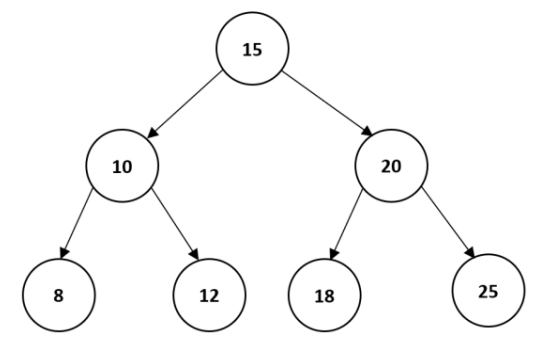
\includegraphics[width=0.25\paperwidth]{C:/Users/Admin/Desktop/Github/question_bank/LyX/static/img/9597-NYJC-2019-P1-Q3-1}
\par\end{center}

The program to implement this ADT will use the classes Tree and Node
designed as follows: 
\begin{center}
\begin{tabular}{|l|}
\hline 
\texttt{ToDo}\tabularnewline
\hline 
\texttt{root : Node}\tabularnewline
\hline 
\texttt{constructor()}\tabularnewline
\texttt{add(newItem)}\tabularnewline
\texttt{printTreeInOrder()}\tabularnewline
\hline 
\end{tabular}%
\begin{tabular}{|l|}
\hline 
\texttt{Node}\tabularnewline
\hline 
\texttt{key : INTEGER}\tabularnewline
\texttt{left : Node}\tabularnewline
\texttt{right : Node}\tabularnewline
\hline 
\texttt{constructor()}\tabularnewline
\texttt{insert(key : INTEGER)}\tabularnewline
\hline 
\end{tabular}
\par\end{center}

\subsection*{Task 3.1 }

Write program code to define the classes \texttt{Tree} and \texttt{Node}.

\subsection*{Evidence 8: }

Your program code. \hfill{}{[}16{]}

\subsection*{Task 3.2 }
\begin{itemize}
\item Write program code for a procedure \texttt{CreateTreefromArray} that
accepts an array of unsorted unique integers passed in via a parameter. 
\item The procedure will read each integer in the array and construct a
binary tree using your classes \texttt{Tree} and \texttt{Node}. 
\item Call \texttt{printTreeInOrder} to display the output (numbers shown
will always be sorted). 
\item Test your program by copying the input data found in \texttt{BST.txt}
into your code. 
\end{itemize}

\subsection*{Evidence 9: }

Your \texttt{CreateTreefromArray} program code. \hfill{}{[}4{]}

\subsection*{Evidence 10: }

A screenshot of the output. \hfill{}{[}2{]}

\subsection*{Task 3.3}

A binary tree created from keys that are in ascending order will result
in an unbalanced binary tree.

For instance, the sequence of commands
\noindent \begin{center}
\begin{tabular}{l}
Create a new tree \tabularnewline
Add to tree (8) \tabularnewline
Add to tree (10) \tabularnewline
Add to tree (12) \tabularnewline
Add to tree (15)\tabularnewline
Add to tree (18) \tabularnewline
Add to tree (20)\tabularnewline
Add to tree (25)\tabularnewline
\end{tabular}
\par\end{center}

will result in a tree that looks as follows: 
\begin{center}
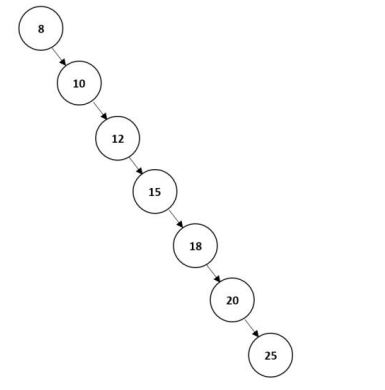
\includegraphics[width=0.25\paperwidth]{C:/Users/Admin/Desktop/Github/question_bank/LyX/static/img/9597-NYJC-2019-P1-Q3-2}
\par\end{center}

Amend procedure \texttt{CreateTreefromArray} so that the created tree
from any input array of integers will be balanced where the number
of items on the left and right subtree will roughly be divided equally
(Hint: input array must first be sorted).

\subsection*{Evidence 11: }

Your amended program code. \hfill{}{[}6{]}

\subsection*{Task 3.4 }

Create a function \texttt{FindKthSmallest} that returns the $k$th
smallest element in your binary tree. If $k=5$ the $k$th smallest
element will be 18. Your function should not need to use extra space
(e.g. creating a new array) to solve the problem other than using
a temp variable(s). 

\subsection*{Evidence 12: }

Your program code for \texttt{FindKthSmallest}. \hfill{}{[}4{]}

\subsection*{Evidence 13:}

Produce a screenshot showing the retrieval of the 5th smallest element
from the tree created earlier. \hfill{}{[}2{]}

{[}SPLIT\_HERE{]}
\item \textbf{{[}NYJC/PRELIM/9597/2019/P1/Q4{]} }

To encrypt a message, a keyword cipher is used. It is a form of monoalphabetic
substitution where a keyword is used as the key. The key is used to
determine the letter matchings of the cipher alphabet to the plain
alphabet. Repeating letters in the key is removed. For instance, if
the key used is \texttt{'SECRET'}, the cipher alphabet generated will
be as follows: 

\begin{tabular}{lcccccccccccccccccccccccccc}
Plain text: & \texttt{A} & \texttt{B} & \texttt{C} & \texttt{D} & \texttt{E} & \texttt{F} & \texttt{G} & \texttt{H} & \texttt{I} & \texttt{J} & \texttt{K} & \texttt{L} & \texttt{M} & \texttt{N} & \texttt{O} & \texttt{P} & \texttt{Q} & \texttt{R} & \texttt{S} & \texttt{T} & \texttt{U} & \texttt{V} & \texttt{W} & \texttt{X} & \texttt{Y} & \texttt{Z}\tabularnewline
Cipher Alphabet: & \texttt{S} & \texttt{E} & \texttt{C} & \texttt{R} & \texttt{T} & \texttt{A} & \texttt{B} & \texttt{D} & \texttt{F} & \texttt{G} & \texttt{H} & \texttt{I} & \texttt{J} & \texttt{K} & \texttt{L} & \texttt{M} & \texttt{N} & \texttt{O} & \texttt{P} & \texttt{Q} & \texttt{U} & \texttt{V} & \texttt{W} & \texttt{X} & \texttt{Y} & \texttt{Z}\tabularnewline
\end{tabular}

After the key\textquoteright s unique letters is used up, the rest
of the ciphertext letters are used in alphabetical order, excluding
those already used in the key. Thus, to encode the word \textquoteleft \texttt{Attack}\textquoteright ,
\textquoteleft \texttt{A}\textquoteright{} is replaced with \texttt{'S'},
\texttt{'t'} is replaced with \texttt{'Q'}, and so on giving the encrypted
word as \texttt{'SQQSCH'}. 

\subsection*{Task 4.1 }

Write program code for a function to generate an array of the cipher
alphabet given a key. 
\noindent \begin{center}
\texttt{FUNCTION Cipher (NewAlphabet : ARRAY, Key : STRING) }
\par\end{center}

The function has two parameters and returns the \texttt{NewAlphabet}
array with the correct cipher alphabet based on the \texttt{Key} parameter. 

\subsection*{Evidence 14:}

Your program code. \hfill{} {[}6{]}

\subsection*{Task 4.2 }

Write driver code that asks the user to enter a key that contains
only letters, calls function Cipher and displays the cipher alphabet
(all in uppercase) in one line. Do appropriate data validation on
the input key. 

\subsection*{Evidence 15: }

Your program code. \hfill{} {[}3{]}

\subsection*{Task 4.3 }

Design three suitable test cases and provide screenshot evidence for
your testing. 

\subsection*{Evidence 16: }

Annotated screenshots for each test data run. \hfill{} {[}3{]}

\subsection*{Task 4.4 }

Develop your program further to display the following menu: 
\begin{enumerate}
\item[1.]  Encode a message
\item[2.]  Decode a message 
\item[3.]  -1 to Quit
\end{enumerate}
Implement the menu options to allow a line of text to be encoded or
decoded. For each option, ask for the cipher key and the message that
is to be encoded or decoded. Test your program with the key \texttt{'TOPSECRET'}
and the message \texttt{'I will score A for Computing}'. 

\subsection*{Evidence 17: }

Your program code. \hfill{}{[}10{]}

\subsection*{Evidence 18: }

Screenshot(s) showing your output. \hfill{}{[}2{]}

\subsection*{Task 4.5 }

Frequency analysis is a common method used by code breakers to break
monoalphabetic substitution ciphers. The first step is to analyse
the coded message and construct a frequency table of all the letters
appearing in the coded message. 

Write a program that reads the content from the file \texttt{INTERCEPT.txt}.
The text in this file contains a coded message. Construct a frequency
table (ignore punctuation marks) as follows using a suitable data
structure: 

\begin{tabular}{lcccccccccccccccccccccccccc}
Ciphertext Letter: & \texttt{A} & \texttt{B} & \texttt{C} & \texttt{D} & \texttt{E} & \texttt{F} & \texttt{G} & \texttt{H} & \texttt{I} & \texttt{J} & \texttt{K} & \texttt{L} & \texttt{M} & \texttt{N} & \texttt{O} & \texttt{P} & \texttt{Q} & \texttt{R} & \texttt{S} & \texttt{T} & \texttt{U} & \texttt{V} & \texttt{W} & \texttt{X} & \texttt{Y} & \texttt{Z}\tabularnewline
Frequency: & \texttt{5} & \texttt{2} & $\cdots$ &  &  &  &  &  &  &  &  &  &  &  &  &  &  &  &  &  &  &  &  &  &  & \tabularnewline
\end{tabular}

Your program will then display the table sorted by descending order
showing the most used letter and its frequency first followed by the
next highest and so on.

Partial sample output: 

\begin{tabular}{lcccc}
Ciphertext Letter: & \texttt{S} & \texttt{O} & \texttt{G} & \texttt{$\cdots$}\tabularnewline
Frequency: & \texttt{88} & \texttt{85} & \texttt{67} & $\cdots$\tabularnewline
\end{tabular}

\subsection*{Evidence 19: }

Your program code. \hfill{} {[}7{]}

\subsection*{Evidence 20: }

Screenshot of output. \hfill{}{[}1{]}

{[}SPLIT\_HERE{]}
\item \textbf{{[}NYJC/PRELIM/9597/2019/P2/Q1{]} }
\begin{enumerate}
\item Database management systems are aimed at solving a number of problems
associated with traditional file-based systems. Describe three such
problems and explain how they are solved by database management systems.
\hfill{} {[}6{]}
\item A national car hire company uses a relational database. Cars are available
for hire from a large number of depots around the country. Two entities
(or records) are CARS-FOR-HIRE and DEPOTS.
\begin{enumerate}
\item Suggest four attributes (or fields) associated with the entity CARS-FOR-HIRE.
\hfill{}{[}4{]}
\item Draw a diagram showing the relationship between the entities CARS-FOR-HIRE
and DEPOTS. \hfill{}{[}1{]}
\item State one other entity which is related to either or both of the original
entities. Describe the relationship(s). Suggest an attribute for this
entity. \hfill{}{[}4{]}
\end{enumerate}
\end{enumerate}
{[}SPLIT\_HERE{]}
\item \textbf{{[}NYJC/PRELIM/9597/2019/P2/Q2{]} }

A stack is to be implemented using an array of 20 elements. 
\begin{enumerate}
\item Describe an algorithm to remove an item from a stack and place it
in a variable \texttt{x}. \hfill{}{[}4{]}
\item With the aid of examples, explain what nested functions or nested
subroutines are. \hfill{} {[}3{]}
\item Explain with the aid of diagrams or otherwise, how a stack can be
used by the operating system to process \textquotedblleft nested functions\textquotedblright{}
or \textquotedblleft nested subroutines\textquotedblright . \hfill{}{[}5{]}
\item Outline the data attributes and member functions for a class stack
abstract data type. You need not go into details as to how they will
be implemented. \hfill{}{[}6{]}
\end{enumerate}
{[}SPLIT\_HERE{]}
\item \textbf{{[}NYJC/PRELIM/9597/2019/P2/Q3{]} }

A large national electrical appliances company maintains an extensive
inventory of appliances for sale in a country. The company has twelve
specialised retail stores targeting the needs of different market
segments. Six of these stores are housed in a large mall in the capital,
but the other six are in different cities in the country. 

The six stores in the capital are linked using a LAN, while the other
six are linked via a WAN. 
\begin{enumerate}
\item Explain the difference between a LAN and a WAN. \hfill{} {[}2{]}
\item Wireless technology has become more popular in recent years. Describe
two reasons why the company will not replace its LAN network with
a wireless one. \hfill{} {[}4{]}
\item Discuss two security threats faced by the company\textquoteright s
LAN and measures that can be put in place to reduce these threats.
\hfill{} {[}6{]}
\end{enumerate}
The company is thinking of allowing all its sales personnel access
to this inventory. It can store this data on an intranet or cloud
storage. Discuss the relative merits and demerits of these two options.
\hfill{}{[}6{]}

{[}SPLIT\_HERE{]}
\item \textbf{{[}NYJC/PRELIM/9597/2019/P2/Q4{]} }

A company has decided to offer an in-house credit system by issuing
privileged customers an in-house credit-card which allows customers
to charge their purchases from the stores to the card, up to the customers\textquoteright{}
credit limits.
\begin{enumerate}
\item During a sales promotion, the store offers a discount of 15\% if a
customer\textquoteright s total purchase is greater or equal to \$200
but less than \$500. A discount of 20\% is given if the customer\textquoteright s
total purchase is greater or equal to \$500. For customers who had
exceeded their credit limits, the supervisor\textquoteright s approval
is required. Create a decision table or tree to represent the above
conditions and actions. \hfill{}{[}5{]}
\item In order to protect the privacy of data, many countries have passed
legislation to address this issue. Describe any 3 features of the
Personal Data Protection Act in Singapore that aims to do this. \hfill{}{[}6{]}
\end{enumerate}
{[}SPLIT\_HERE{]}
\item \textbf{{[}NYJC/PRELIM/9597/2019/P2/Q5{]} }

When a customer orders goods over the phone, the cashier will record
the order in an order form containing the items ordered and quantity,
customer address, delivery date and time and the amount payable. A
copy of this form will be given to the storeman who will pick the
goods and generate a delivery order (DO). The DO will be given to
the delivery man who will deliver the goods. The customer on collecting
the goods will sign on the DO and return a signed copy to the delivery
man. On his return, the delivery man will give the DO to the accounts
department who will generate an invoice. Invoices are kept in a file
until the next day where they will be mailed to the customers.
\begin{enumerate}
\item Draw a data flow diagram of the above processes.\hfill{} {[}8{]} 
\item Goods in the warehouse are divided into 2 main categories -- Kitchen
appliances (e.g. kettle, toasters and ovens) and Entertainment products
(e.g. LCD television, mp3 players and gaming consoles). Each item
has an item name, description, unit price and quantity on hand. Kitchen
appliances have an item weight, packing volume and colour. Entertainment
products have a serial number, country of manufacture and recommended
retail price.
\begin{enumerate}
\item Draw a class diagram of the above showing inheritance, their private
attributes and public methods.\hfill{} {[}6{]}
\item What is the purpose of a public method?\hfill{} {[}1{]}
\item What is the difference between a class and an object?\hfill{} {[}2{]}
\end{enumerate}
\item In relation to the diagram in part (b), explain the terms: 
\begin{enumerate}
\item Encapsulation; \hfill{}{[}2{]}
\item Inheritance;\hfill{} {[}2{]}
\item Data hiding; \hfill{}{[}2{]}
\item Polymorphism. \hfill{}{[}2{]}
\end{enumerate}
\end{enumerate}
{[}SPLIT\_HERE{]}
\item \textbf{{[}NYJC/PRELIM/9597/2019/P2/Q6{]} }

A linked list ADT with the following incomplete specification is given
as follows:
\begin{center}
\begin{tabular}{|l|}
\hline 
\texttt{LList}\tabularnewline
\hline 
\texttt{head : Node}\tabularnewline
\hline 
\texttt{constructor()}\tabularnewline
\texttt{addNode(s : Node)}\tabularnewline
\texttt{findmiddle(l : llist)-> INTEGER}\tabularnewline
\hline 
\end{tabular}%
\begin{tabular}{|l|}
\hline 
Node\tabularnewline
\hline 
\texttt{data : INTEGER}\tabularnewline
\texttt{nextPtr : Node}\tabularnewline
\hline 
\texttt{constructor()}\tabularnewline
\texttt{setData(s : INTEGER)}\tabularnewline
\texttt{setnextPtr(x : Node)}\tabularnewline
\texttt{getData(): INTEGER }\tabularnewline
\hline 
\end{tabular}
\par\end{center}
\begin{enumerate}
\item Explain the main difference between an array and a linked list data
structure.\hfill{} {[}2{]}
\item Using pseudo code, write an algorithm to implement \texttt{findmiddle}
that will return the data in the middle of the linked list in one
pass. \hfill{}{[}7{]}
\item State two applications of a linked list. \hfill{}{[}2{]}
\item State two other common methods (including parameters) that should
be included in the \texttt{LList} specification.\hfill{} {[}2{]}
\end{enumerate}
{[}SPLIT\_HERE{]}
\end{enumerate}

\end{document}
